\documentclass[a4paper, 12pt]{report}
\usepackage{hyperref}
\usepackage[utf8]{inputenc} % выбор кодировки кода
\usepackage[T1, T2A]{fontenc} % выбор внутренней кодировки 
\usepackage[english, russian]{babel} % выбор языка
% \righthyphenmin = 2 % минимальное число букв после переноса: может пригодиться
\usepackage{amsmath} % русский текст в формулах
\usepackage{color} % цвет текста
\usepackage{ulem} % для зачёркивания текста

\usepackage[left=15mm, right=10mm, top=20mm, bottom=20mm]{geometry} % поля
\usepackage{indentfirst} % отступ первого абзаца
\setlength{\parindent}{1,25cm} % длина отступа первой строки абзаца
\linespread{1,5} % междустрочный интервал

\usepackage{titlesec} % настройка заголовков
\renewcommand{\thesection}{\arabic{section}} % противотараканная мера для report'а: делаю section заголовком первого уровня
\titleformat{\section}{\centering \large \bfseries}{\thesection}{1ex}{\MakeUppercase}{}
\titleformat{\subsection}{\centering \large \bfseries}{\thesubsection}{1ex}{}{}
\titleformat{\subparagraph}[runin]{\bfseries}{\thesubparagraph}{}{}{}
% \titleformat{\bibliography}{\centering \large \bfseries}{\thebibliography}{}{}{} % попытка настроить заголовок для списка литературы

\usepackage{graphicx}
\graphicspath{{./Photos/}}


\usepackage{comment} % Для многострочных комментариев
\usepackage{xcolor} % Для девочек 



\begin{document}
\begin{titlepage}
\setlength\parindent{0pt}
	\begin{center}
		\large{РОО <<Федерация спортивного туризма Московской области>>\\
		ОО г. Долгопрудного <<Федерация спортивного туризма>>\\}
	\end{center}

	


	
	\begin{center}
		
\includegraphics[width=0.4\linewidth]{../pics/Flag_GS-2}
		
		\Large{\bfseries{ОТЧЁТ}} \\
		\normalsize о прохождении горного спортивного туристического маршрута \textbf{первой} категории сложности по Западному Кавказу (Гвандра), совершённом с 18 по 30 августа 2024 г. группой туристов Горной секции МФТИ ФСТ Московской области, г. Долгопрудный
	\end{center}
	\vspace{1.5 cm}
	
	\textbf{Маршрутная книжка:} 41/2024, выдана МКК ФСТ МО г. Долгопрудный \\ 
	\textbf{Руководитель группы:} Снеговская Дарья Алексеевна\\
	\textbf{E-mail:} \href{mailto: snegovskaya\_da@mail.ru}{snegovskaya\_da@mail.ru}\\
	\textbf{Номер телефона:} $+7(964)599-90-08$
	
	\vspace{0.2cm}
	
	\textit{Маршрутно-квалификационная комиссия Федерации спортивного туризма Московской области рассмотрела отчёт и считает, что маршрут может быть зачтен всем участникам и руководителю \textbf{первой категории сложности}.}

	\vspace{0.2cm}
	
	Отчёт использовать в библиотеке ФСТ Московской области и ФСТ г. Долгопрудный.
	
	\vspace{1cm}
	
	\textbf{Судья по виду:}
	
	\vspace{0.5cm}
	\textbf{Председатель МКК:}
	
	\vspace{1cm}
	\textbf{Штамп МКК:}
	
	\vfill
	\begin{center}
		Долгопрудный,   \the\year{}
	\end{center}
\end{titlepage}

\tableofcontents
\section{Справочные сведения о походе} 
\subsection{Проводящая организация}
Поход был совершён в рамках школы горного туризма базового уровня, организованной Горной секцией МФТИ.


\subsection{Место проведения}
\textbf{Страна:} Россия

\textbf{Субъекты федерации:} КЧР, КБР

\textbf{Район:} Западный Кавказ

\textbf{Подрайоны:} Гвандра, Приэльбрусье

\subsection{Общие справочные сведения о маршруте}

\begin{table}[h!]
	\resizebox{\textwidth}{!}{%
		\begin{tabular}{|c|c|c|cc|c|}
			\hline
			\multirow{2}{*}{\begin{tabular}[c]{@{}c@{}}Дисциплина\\ (вид туризма)\end{tabular}} & \multirow{2}{*}{\begin{tabular}[c]{@{}c@{}}Категория сложности\\ маршрута\end{tabular}} & \multirow{2}{*}{\begin{tabular}[c]{@{}c@{}}Протяжённость\\ активной части, км$^1$\end{tabular}} & \multicolumn{2}{c|}{\begin{tabular}[c]{@{}c@{}}Продолжительность активной\\ части\end{tabular}} & \multirow{2}{*}{Сроки проведения}                                   \\ \cline{4-5}
			&                                                                                         &                                                                                             & \multicolumn{1}{c|}{Общая}                            & Ходовых дней                            &                                                                     \\ \hline
			Горный                                                                              & Первая                                                                                  & 111                                                                                         & \multicolumn{1}{c|}{13}                               & 13                                      & \begin{tabular}[c]{@{}c@{}}18.08.2024-\\ 30.08.2024 г.\end{tabular} \\ \hline
		\end{tabular}%
	}
\end{table}
\footnotesize{$^1$ С учётом коэффициента $k=1.2$, без учёта повторно пройденного пути}
\normalsize

\subsection{Подробная нитка маршрута}
\textbf{Заявленная:} г. Минеральные Воды~--- д.р. Учкулан~--- д.р. Кичкинакол Уллукёльский~--- \textbf{пер. Уллукёль Восточный (1А, 3050)}~--- т/б <<Глобус>>~--- д.р.Гондарай~--- д.р. Джалпаккол~--- \textbf{пер. Джалпаккол Сев. (1А, 3400)}~--- д.р. Мырды~--- а/л<<Узункол>>~--- д.р.Кичкинекол~--- д.р. Таллычат~--- \textbf{пер. Кичкинекол Малый (1А, 3210)}~--- д.р. Чунгур-Джар~--- \textbf{пер. Перемётный (1А, 3242)}~--- д.р. Танышхан~--- д.р. Чиринкол~--- стоянка <<Гвандра>>~--- д. р. Кубань~--- \textbf{пер. Хотютау (1А, 3546)}~--- лед. Большой Азау~--- с. Терскол

\textbf{Пройденная:} Маршрут пройден без изменений.

\textbf{Корнилов Георгий} сошёл с маршрута в т/б <<Глобус>>. Он прошёл перевал Уллукёль Восточный (1А$^{\star}$). \alert{L=??}

\textbf{Миронова Наталья} сошла с маршрута в а/л <<Узункол>>. Она прошла перевалы Уллукёль Восточный (1А$^{\star}$), Джалпаккол Северный (1А$^{\star}$). \alert{L=??}

\textbf{Шалфеев Илья, Мерзликина Дарья, Сингалевич Дмитрий, Семено Мария} сошли с маршрута после д.р. Чиринкол, на погранзаставе <<Хурзук>>. Они прошли перевалы Уллукёль Восточный (1А$^{\star}$), Джалпаккол Северный (1А$^{\star}$), Кичкинекол Малый (1А), Перемётный (1А). \alert{L=??}

\begin{figure}
	\centering
	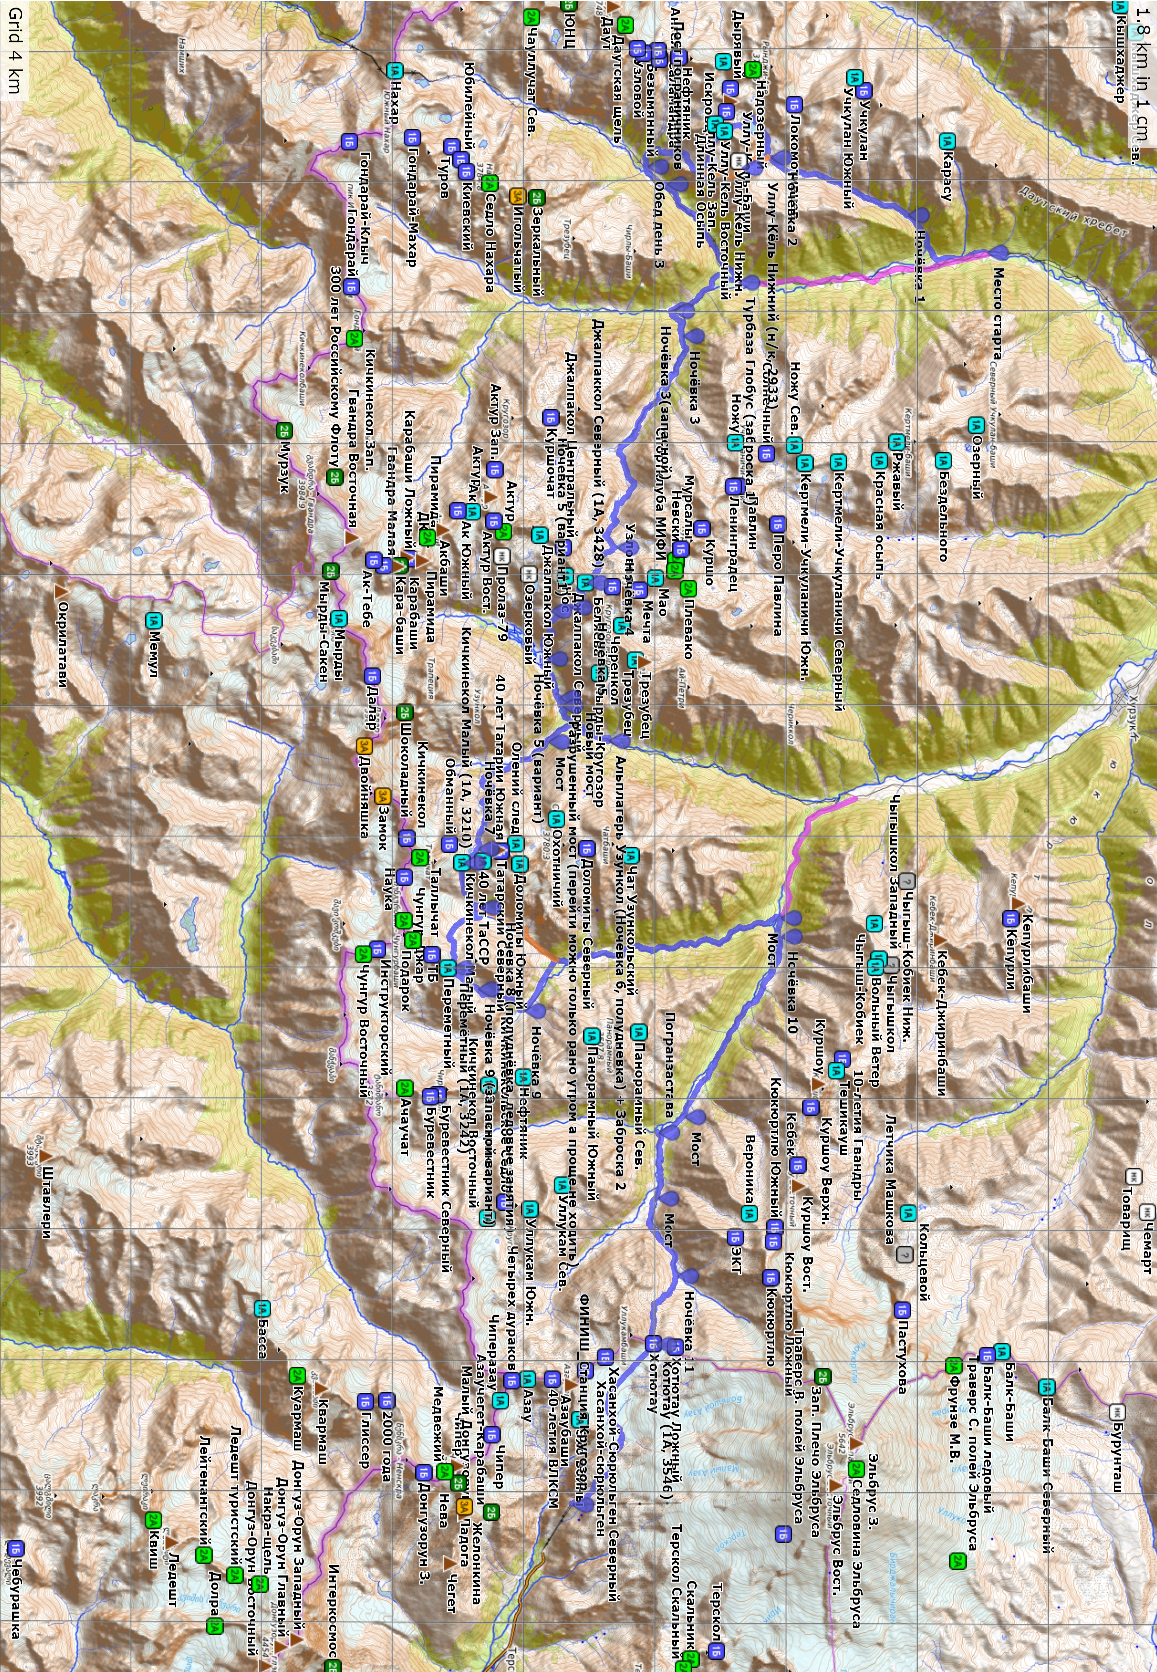
\includegraphics[width=0.92\linewidth]{../pics/map}
	\caption{Обзорная схема маршрута}
\end{figure}
	
\subsection{Высотный профиль маршрута}

\begin{figure}
	\centering
	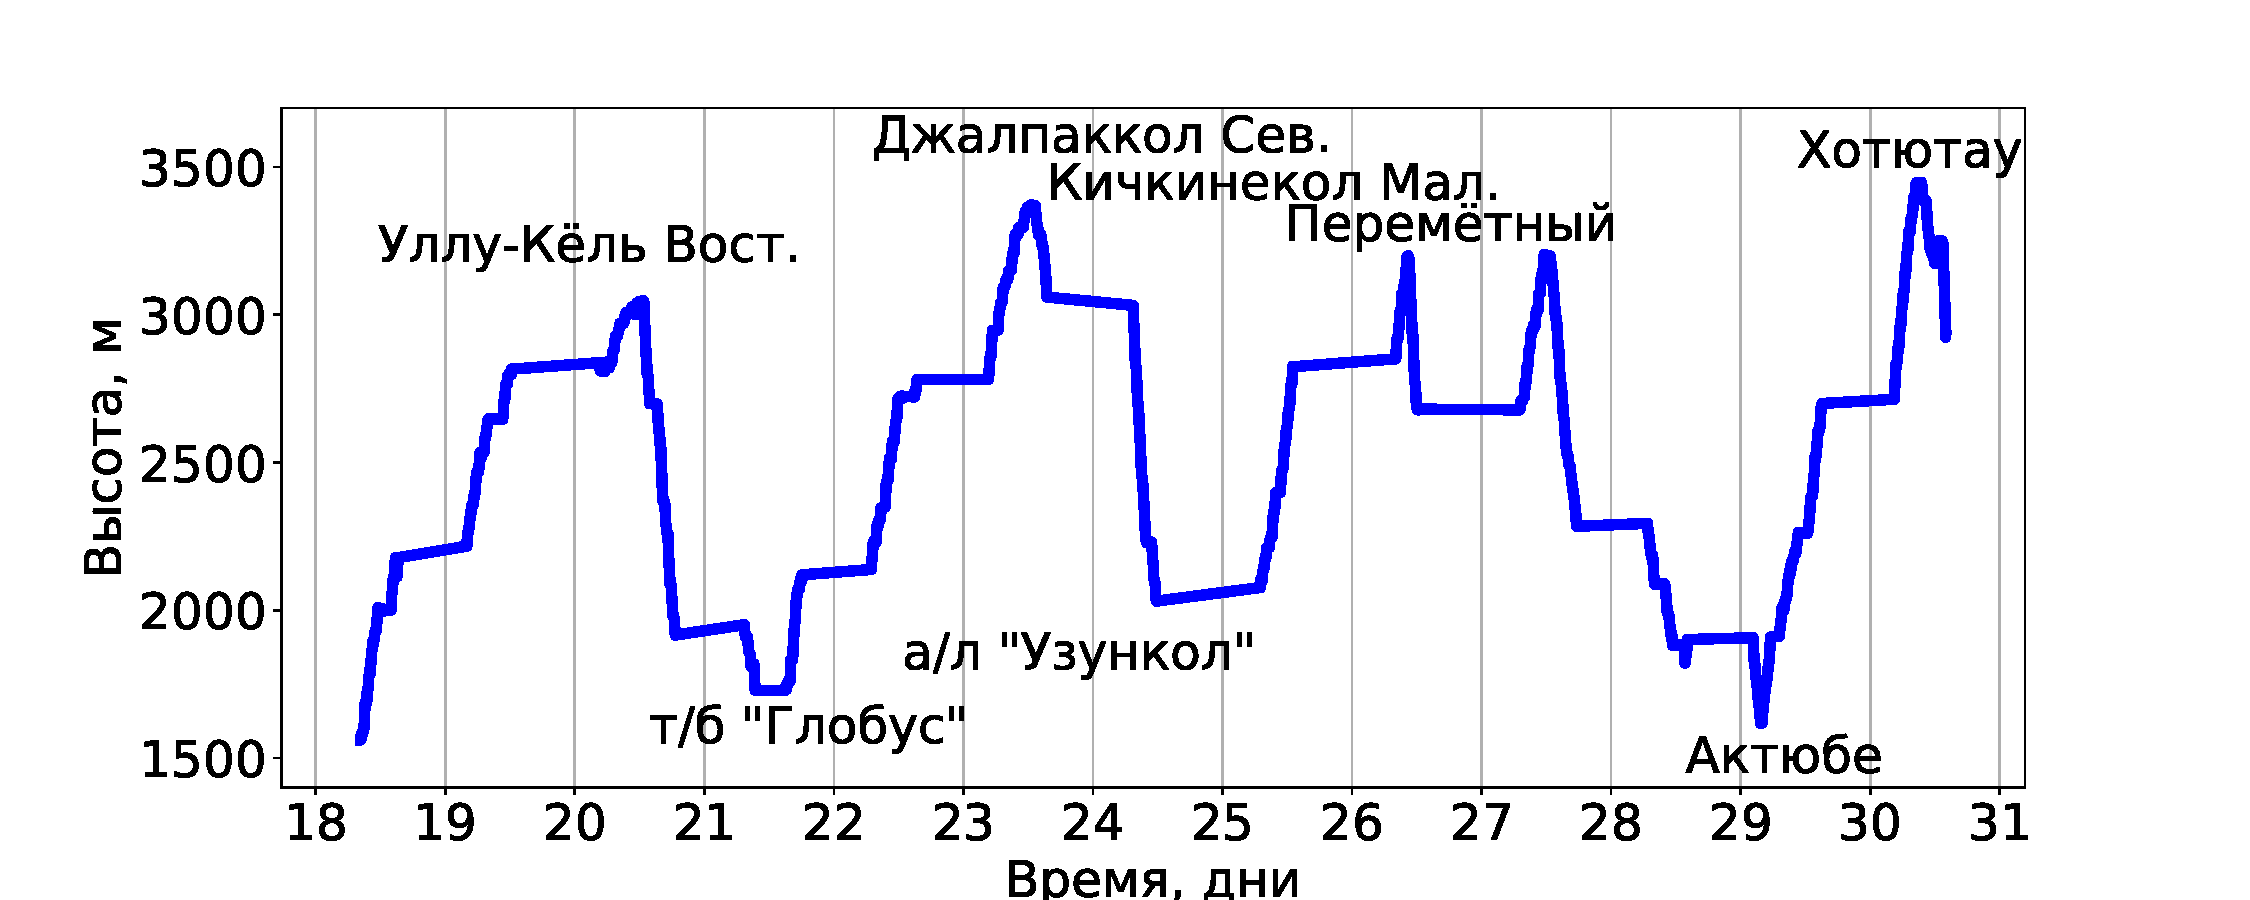
\includegraphics[width=0.92\linewidth]{../pics/elevation_vs_time}
	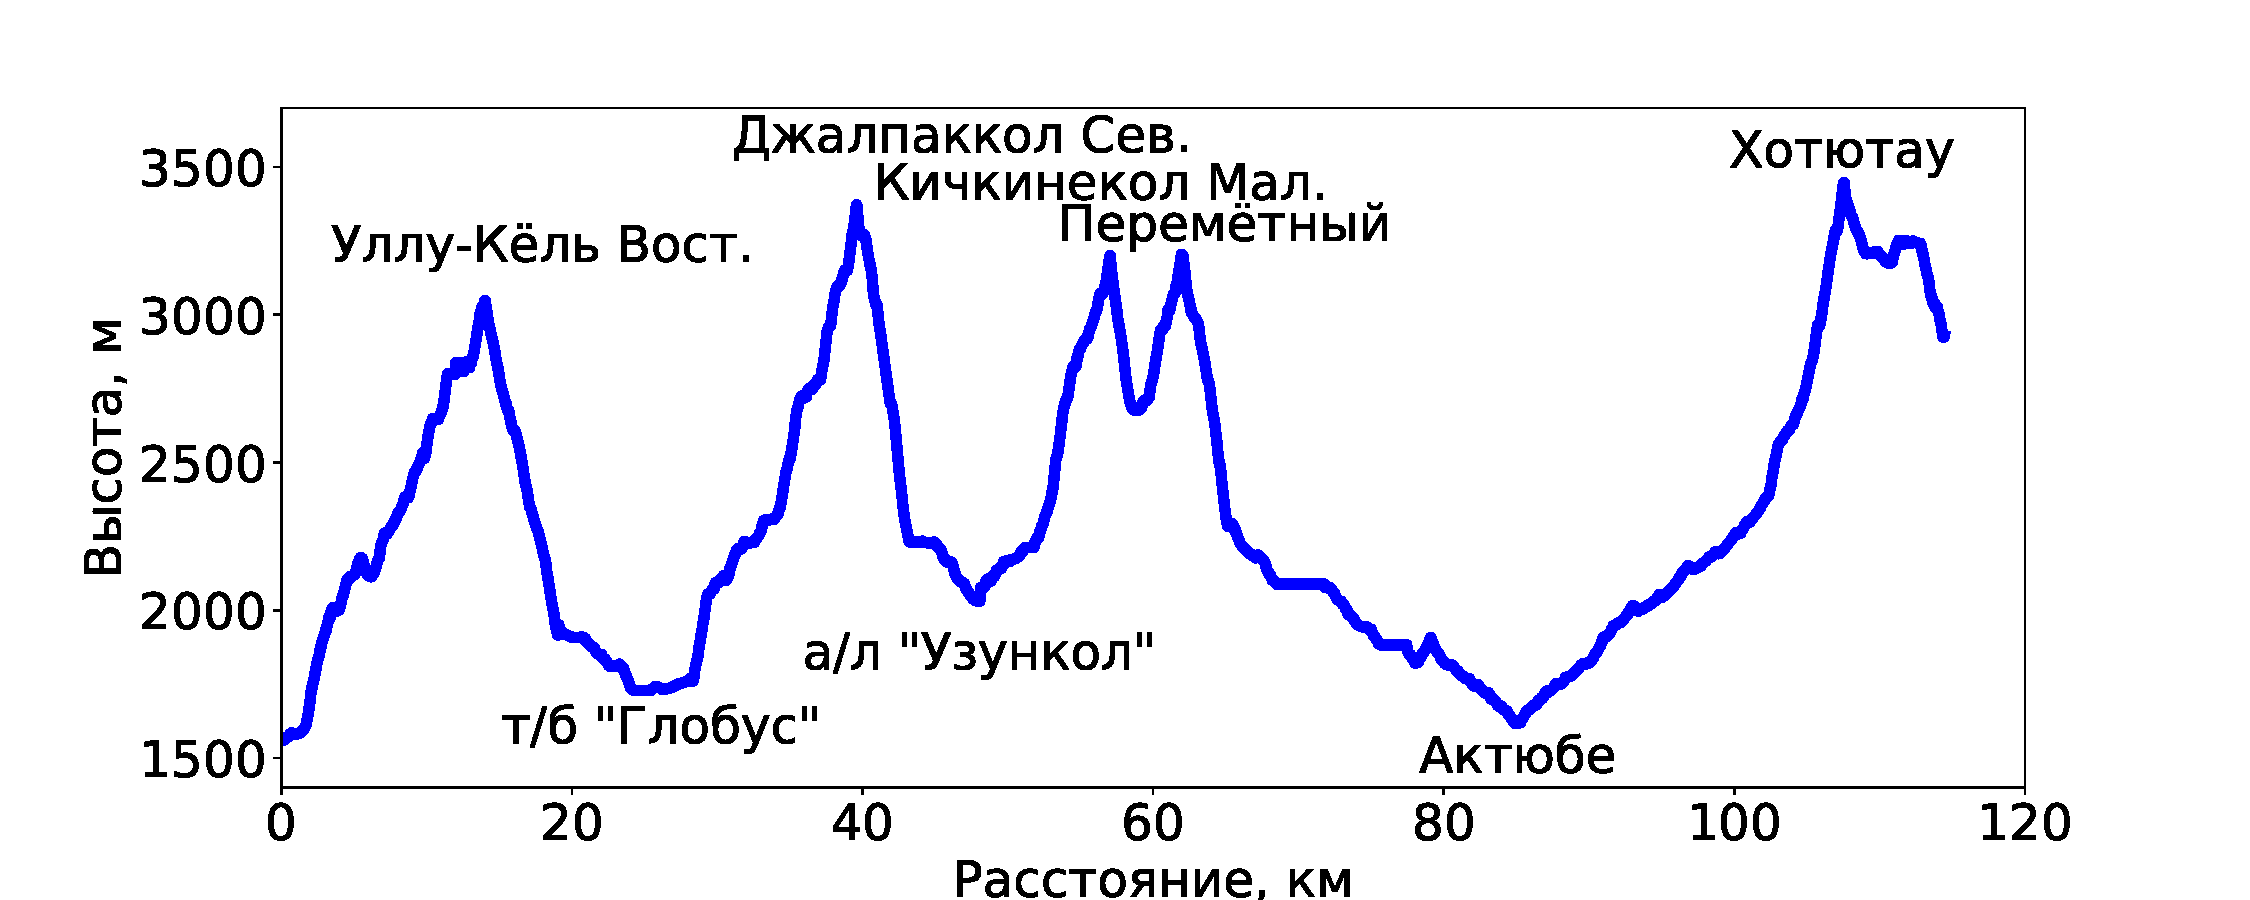
\includegraphics[width=0.92\linewidth]{../pics/elevation_vs_distance}
	\caption{Высотный профиль маршрута}
	\label{fig:heights}
\end{figure}

\subsection{Определяющие препятствия маршрута}

\begin{table}[h!]
		\begin{tabular}{|>{\centering\arraybackslash}m{0.17\linewidth}|>{\centering\arraybackslash}m{0.03\linewidth}|>{\centering\arraybackslash}m{0.4\linewidth}|>{\centering\arraybackslash}m{0.3\linewidth}|}
			\hline
			\textbf{Вид препятствия, высота} &
			\begin{turn}{90}\textbf{к. тр.}\end{turn} &
			\textbf{Характеристика препятствия на подъём} &
			\textbf{Характеристика препятствия на спуск} \\
			\hline			
			пер. Уллу-Кёль Восточный, 3050 & 1А$^{\star}$ &  Со стороны оз. Уллукёль ос. перевальный взлёт протяжённостью до 350 м. У подножия крутизна $20-25^{\circ}$; далее осыпной участок крутизной до $30^{\circ}$ протяжённостью до 100 м и далее снежник крутизной до $35-40^{\circ}$, а в верхней части до $45^{\circ}$, протяжённостью до 50 м. & Движение по гребню до озера под перевалом, далее травяной склон \\
			\hline			
			пер. Джалпаккол Северный, 3411  & 1А$^{\star}$ & Со стороны д.р. Джалпаккол перевальный взлёт лед.-ос. протяжённостью до 200 м, крутизной $35-40^{\circ}$. Выход на перевал — 5 м простого лазания на скальный гребень.  & ск.-ос., протяжённостью до 150 м, крутизной до $30^{\circ}$ \\
			\hline
			пер. Кичкинекол Малый, 3206  & 1А & Со стороны д.р. Кичкинекол по тр.-ос. склону по тропе, протяжённостью до 300 м, крутизной до $25^{\circ}$. На седловине перевала снежник. & ск.-ос. тропа протяжённостью до 200 м., крутизной до $15^{\circ}$\\
			\hline
			пер. Перемётный, 3255  & 1А & Со стороны д.р. Чунгур-Джар перевальный взлёт ск.-ос. протяжённостью до 400 м, крутизной до  $20^{\circ}$ & ск.-ос. склон протяжённостью до 100 м, крутизной до $35^{\circ}$, далее косым траверсом по курумнику. Обход сбросов левее березняка по лощине.\\
			\hline
			пер. Хотютау, 3546  & 1А$^{\star}$ & Со стороны д.р. Уллу-Кам подъём по ос.склону протяжённостью до 1000 м, крутизной до $25^{\circ}$. &  ос. склон протяжённостью до 70 м, крутизной до $30^{\circ}$, выход на открытый ледник\\
			\hline
	\end{tabular}%
\end{table}

\subsection{Список участников} 
Тут будет список наших \sout{долбанов} зайчиков.
\begin{table}[h!]
	\centering
	\resizebox{0.77\textwidth}{!}{%
	\begin{tabular}{|>{\centering\arraybackslash}m{0.02\linewidth}|>{\centering\arraybackslash}m{0.2\linewidth}|>{\centering\arraybackslash}m{0.14\linewidth}|>{\centering\arraybackslash}m{0.05\linewidth}|>{\centering\arraybackslash}m{0.15\linewidth}|>{\centering\arraybackslash}m{0.18\linewidth}|}
		\hline
		\textbf{№} &
		\textbf{Фото} &
		\textbf{ФИО} &
		\textbf{г.р.} &
		\textbf{Обязанности в группе} &
		\textbf{Спортивный опыт} \\
		\hline			
		
		1	&	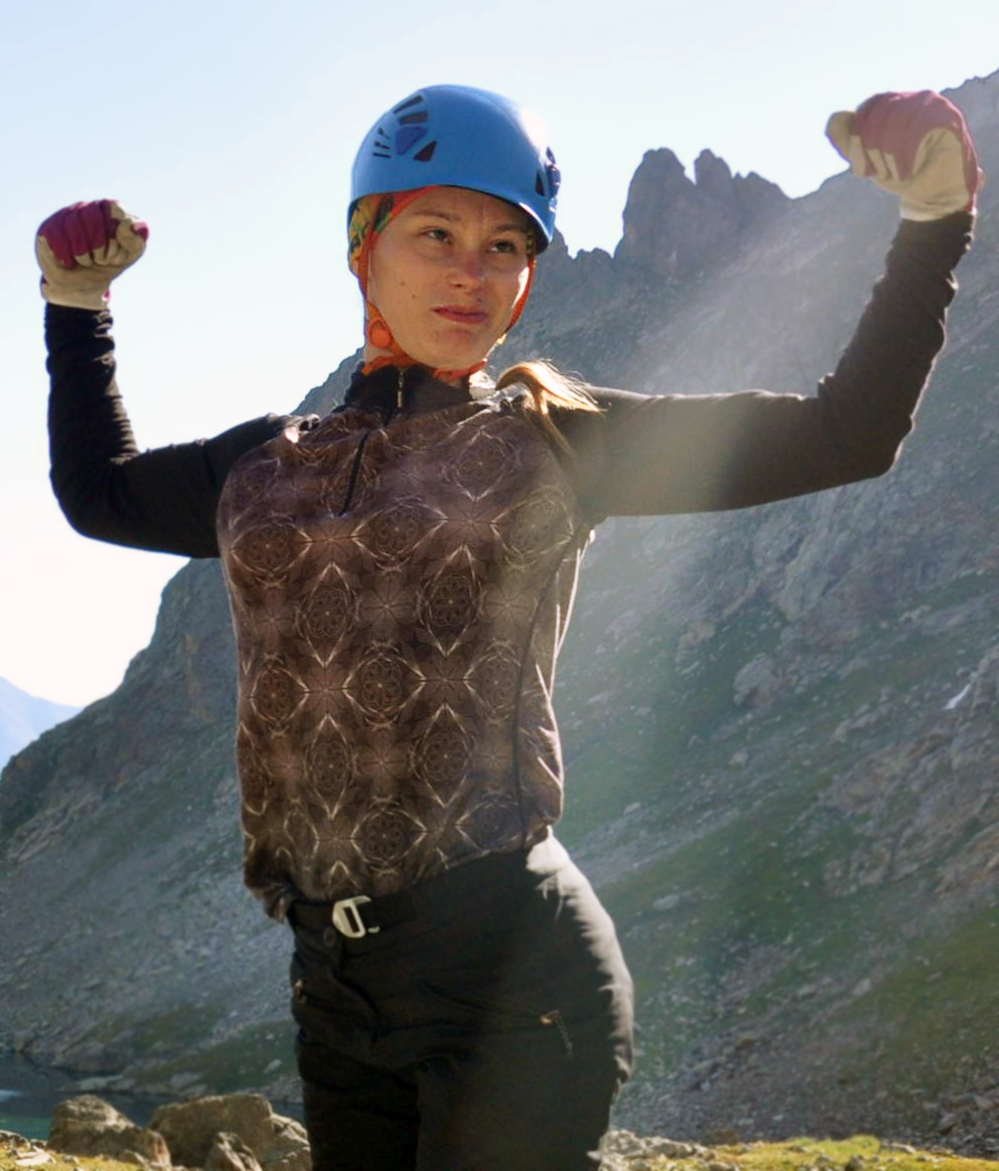
\includegraphics[width=0.99\linewidth]{../pics/portraits/dasha_s.png}	&	Снеговская Дарья Алексеевна	&	1997	&	Руководитель	& 3ГУ, Центральный Кавказ, 2020 \newline 1ГУ, Алтай, Северо-Чуйский хребет, 2023 \\
		\hline
		2	& 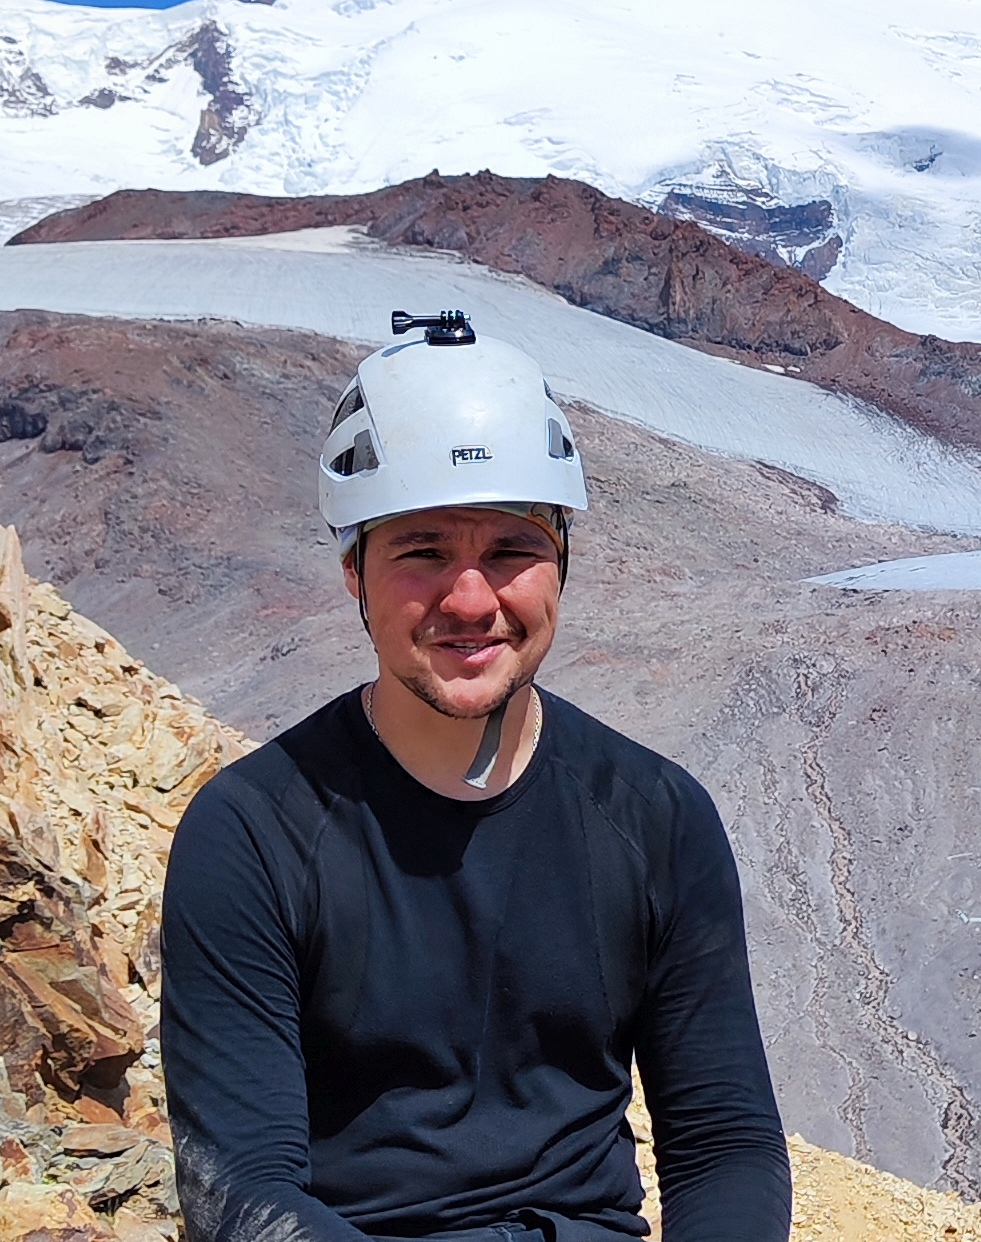
\includegraphics[width=0.99\linewidth]{../pics/portraits/lesha_o1}	&	Остапив Алексей Юрьевич	&	1998	&	Зам. руководителя	& 2ГУ, Киргизский хребет, 2019 \newline 1ГУ, Алтай, Северо-Чуйский хребет, 2023 \\
		\hline
		3	&	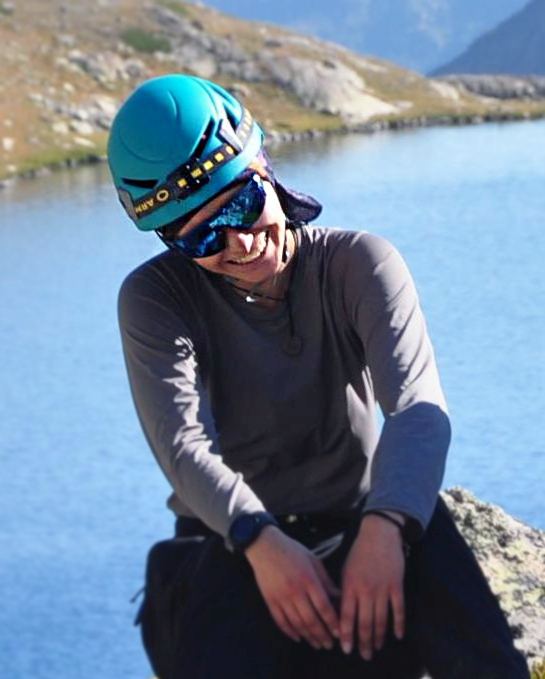
\includegraphics[width=0.99\linewidth]{../pics/portraits/katya}	&	Тюрина Екатерина Алексеевна	&	2004	&	Медик	&	1 ст.с. \\
		\hline
		4	&		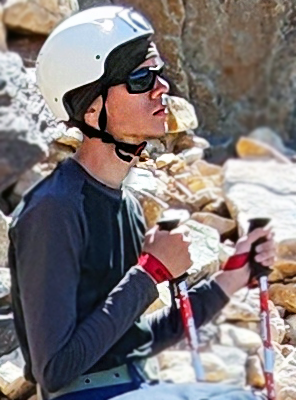
\includegraphics[width=0.99\linewidth]{../pics/portraits/dima_d.png}		&	Дёмушкин .Дмитрий Юрьевич	&	2001	&	Штурман	&	1 ст.с. \\
		\hline
		5	&	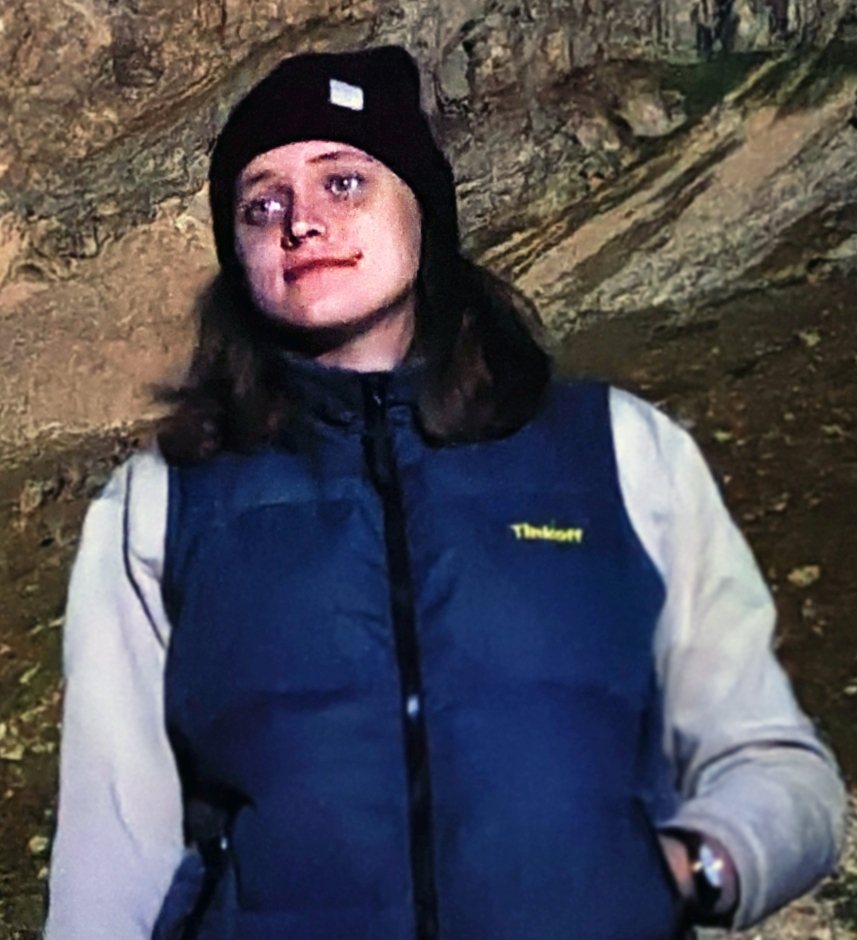
\includegraphics[width=0.99\linewidth]{../pics/portraits/natasha}	&	Миронова Наталья Сергеевна	&	2000	&	Хронометрист	&	1 ст.с. \\
		\hline
		6	&	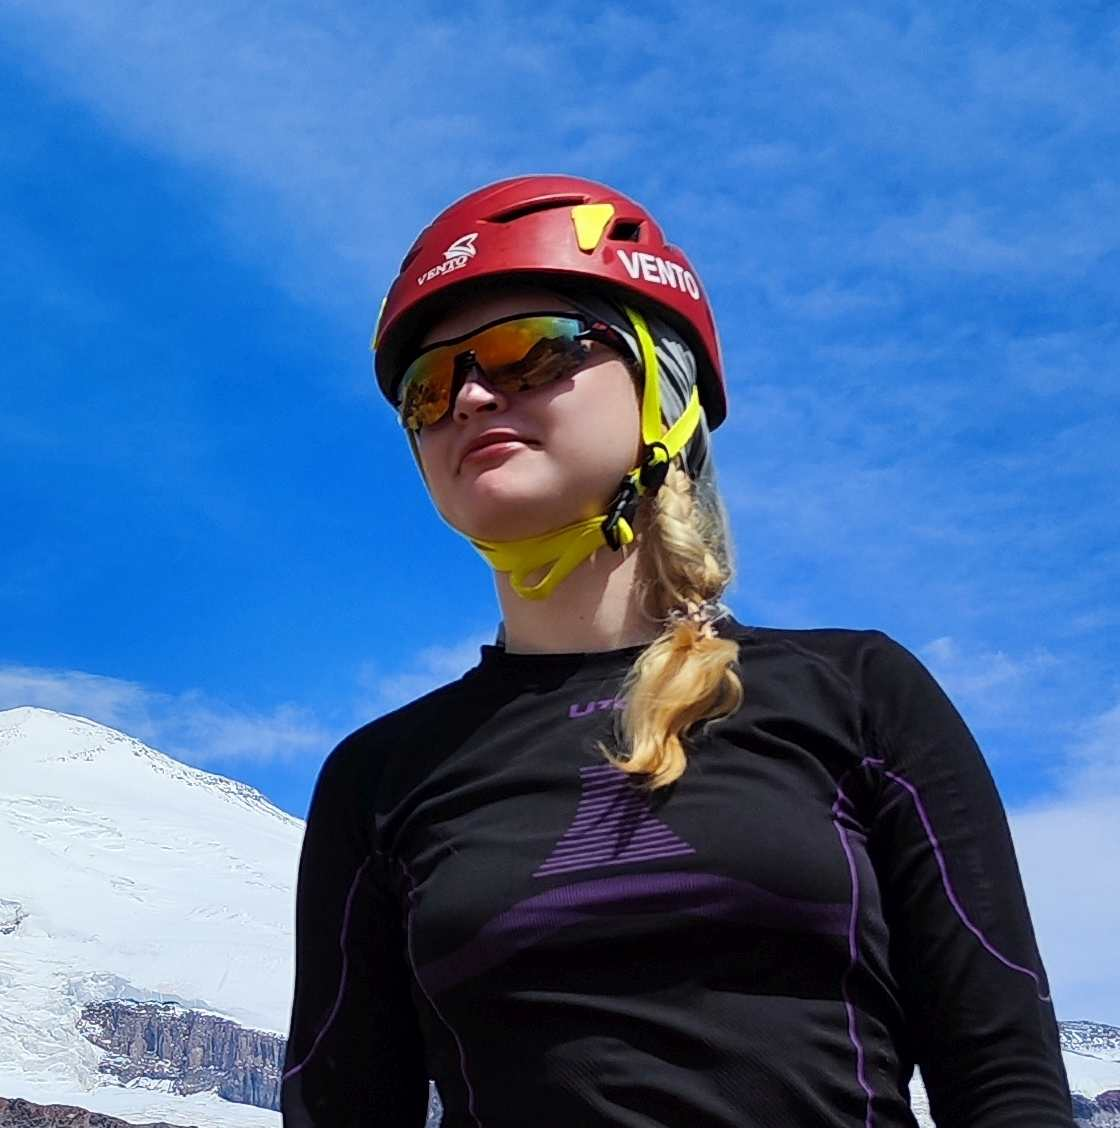
\includegraphics[width=0.99\linewidth]{../pics/portraits/dasha_k}	&	Казаринова Дарья Дмитриевна	&	2001	&	Логист	&	1 ст.с. \\
	\hline
	\end{tabular}%
	}
\end{table}


\begin{table}[h!]
	\centering
	\resizebox{0.75\textwidth}{!}{%
	\begin{tabular}{|>{\centering\arraybackslash}m{0.02\linewidth}|>{\centering\arraybackslash}m{0.2\linewidth}|>{\centering\arraybackslash}m{0.14\linewidth}|>{\centering\arraybackslash}m{0.05\linewidth}|>{\centering\arraybackslash}m{0.15\linewidth}|>{\centering\arraybackslash}m{0.18\linewidth}|}
		\hline
		\textbf{№} &
		\textbf{Фото} &
		\textbf{ФИО} &
		\textbf{г.р.} &
		\textbf{Обязанности в группе} &
		\textbf{Спортивный опыт} \\
		\hline
		7	&	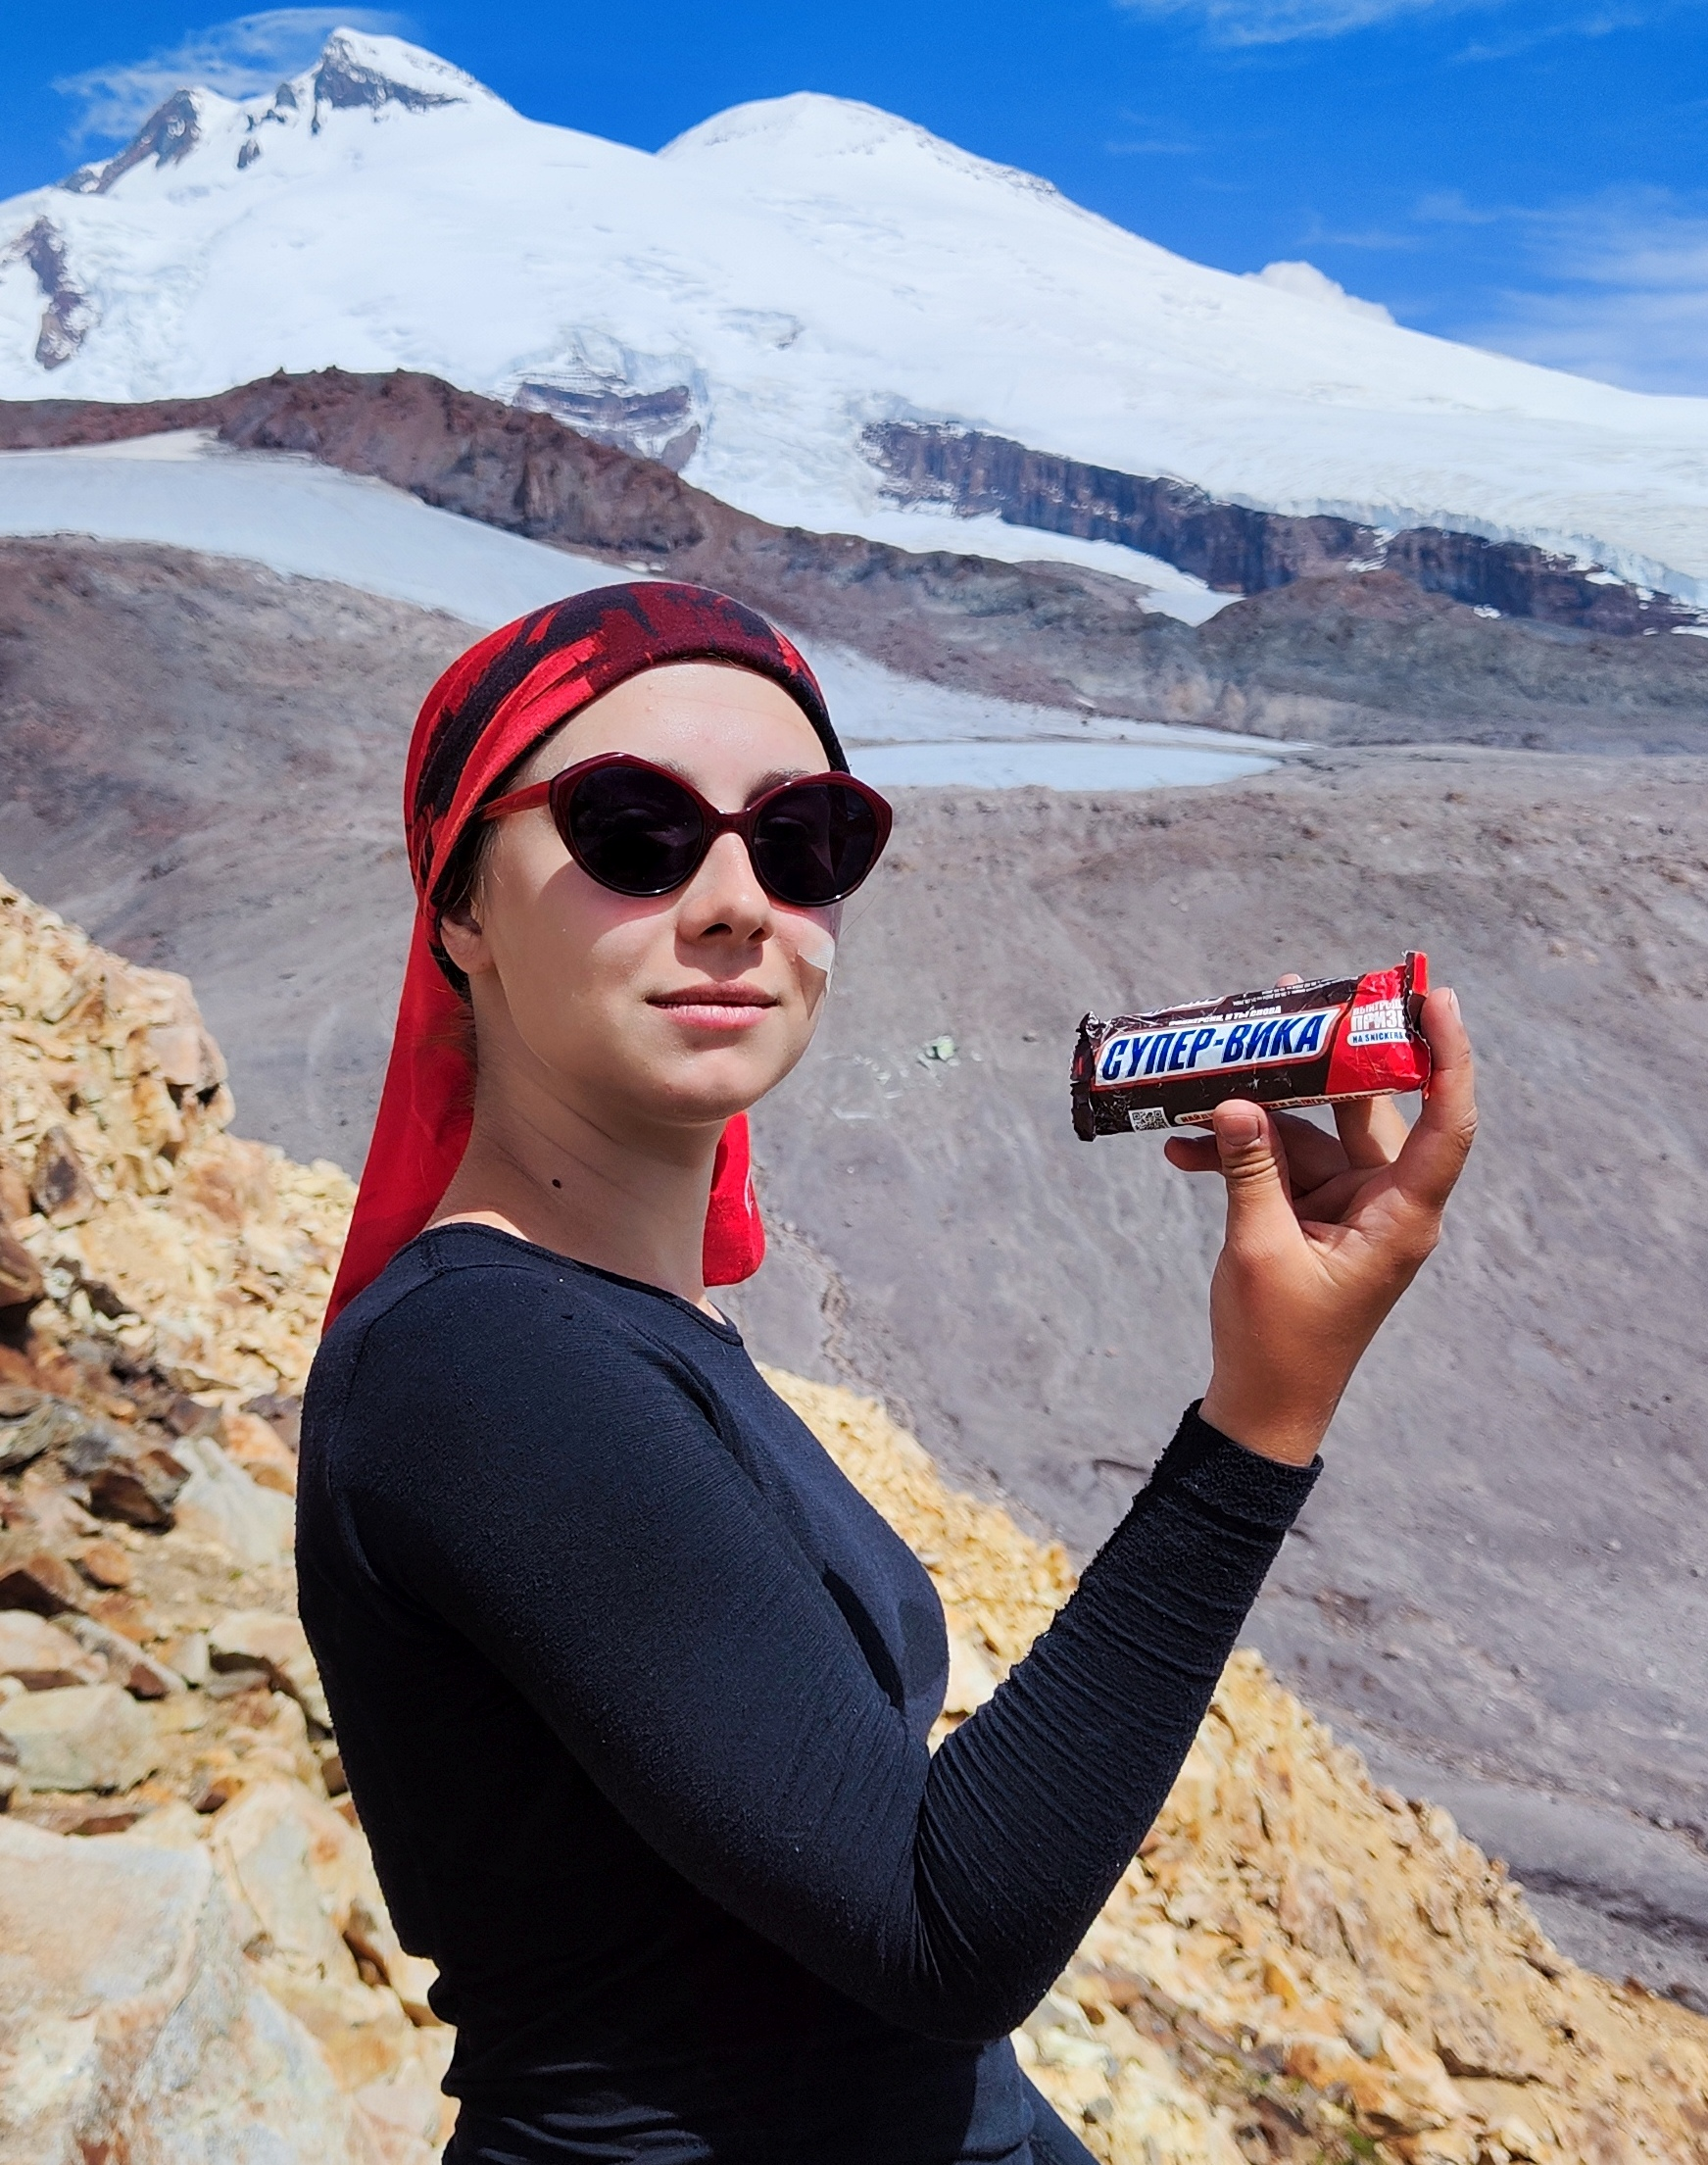
\includegraphics[width=0.99\linewidth]{../pics/portraits/vika}	&	Суровцева Виктория Павловна	&	2002	&	Снаряженец	&	1 ст.с. \\
		\hline
		8	&	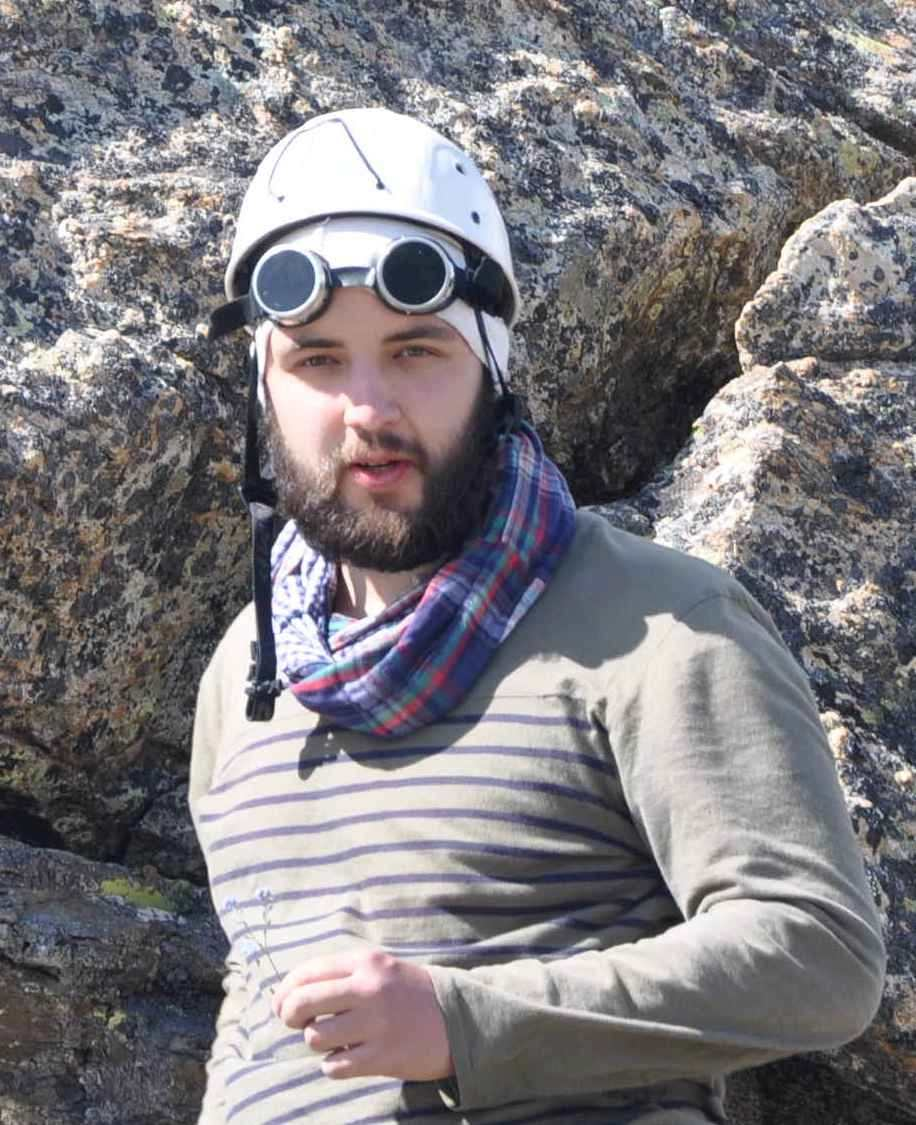
\includegraphics[width=0.99\linewidth]{../pics/portraits/gosha}		&	Корнилов Георгий Алексеевич	&	2003	&	Завхоз 1	&	1 ст.с. \\
		\hline
		9	&	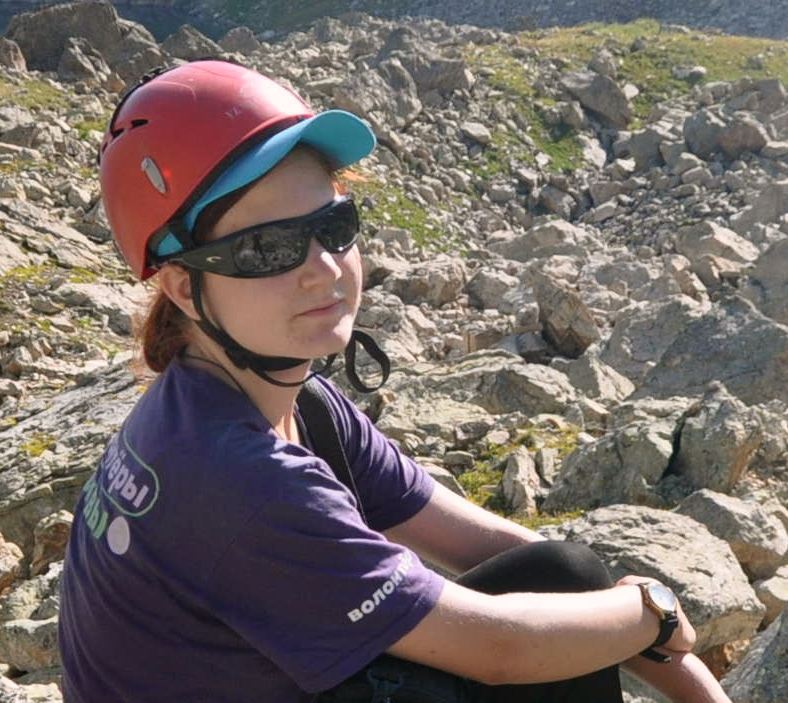
\includegraphics[width=0.99\linewidth]{../pics/portraits/masha}	&	Семено Мария Алексеевна	&	2006	&	Завхоз	2	&	1 ст.с. \\
		\hline
		10	&	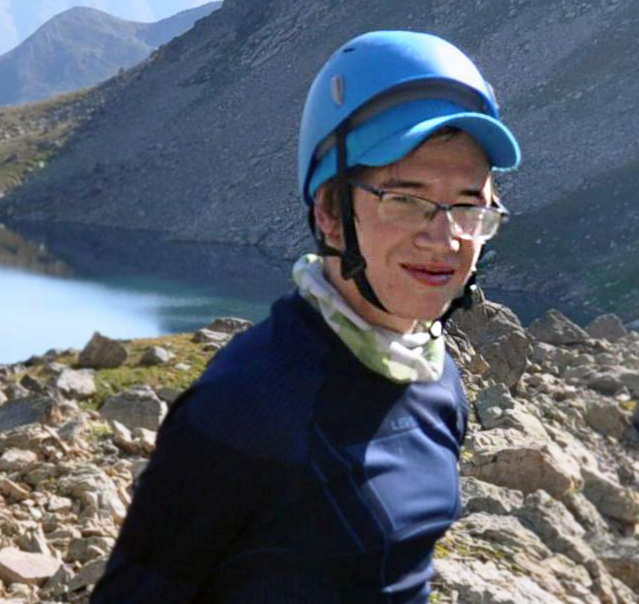
\includegraphics[width=0.99\linewidth]{../pics/portraits/dima_s}	&	Сингалевич Дмитрий Константинович	&	2004	&	Эколог	&	1 ст.с. \\
		\hline
		11	&	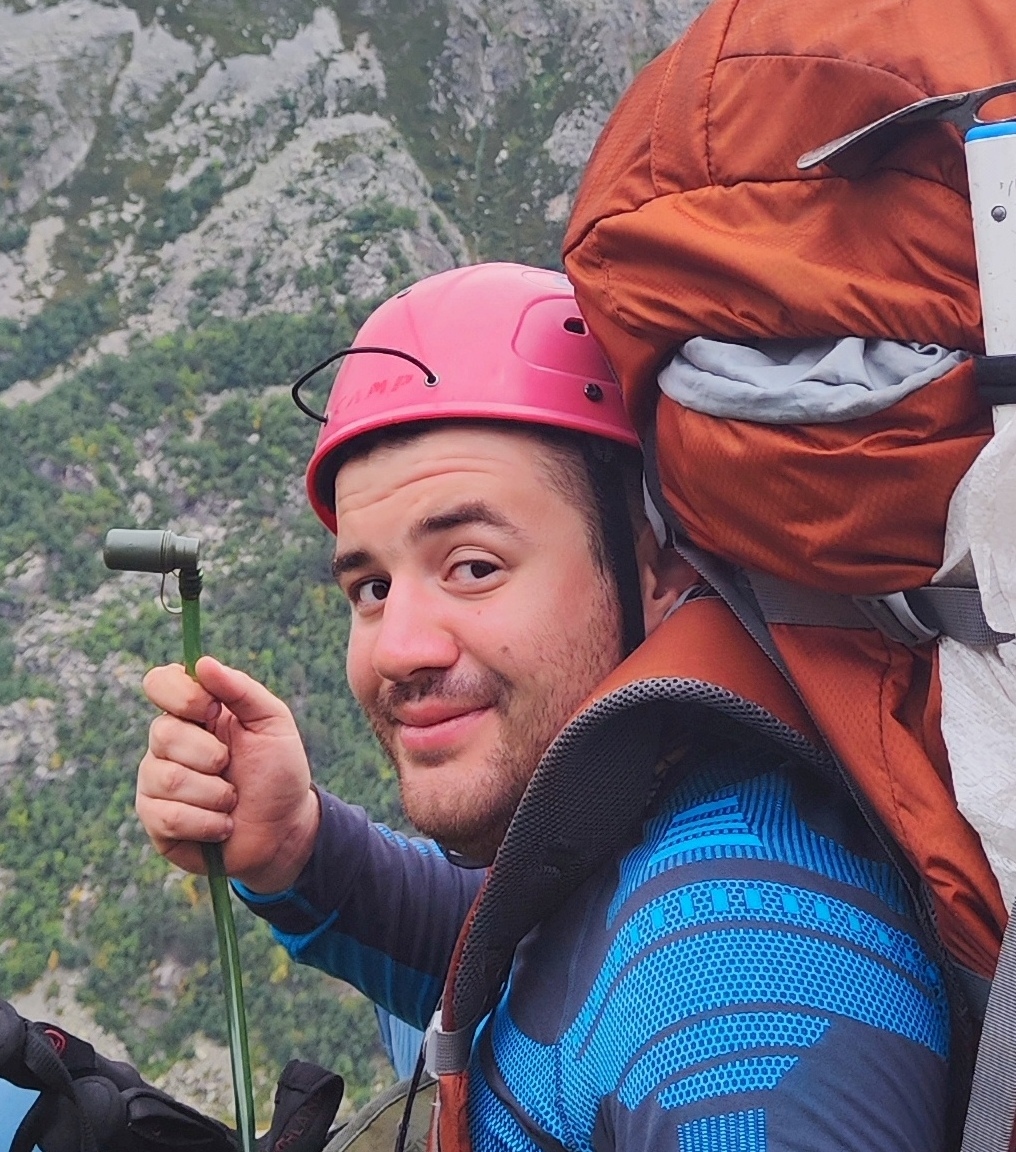
\includegraphics[width=0.99\linewidth]{../pics/portraits/ilya_sh}	&	Шалфеев Илья Андреевич	&	1997	&	Финансист	&	1 ст.с. \\
		\hline
		12	&	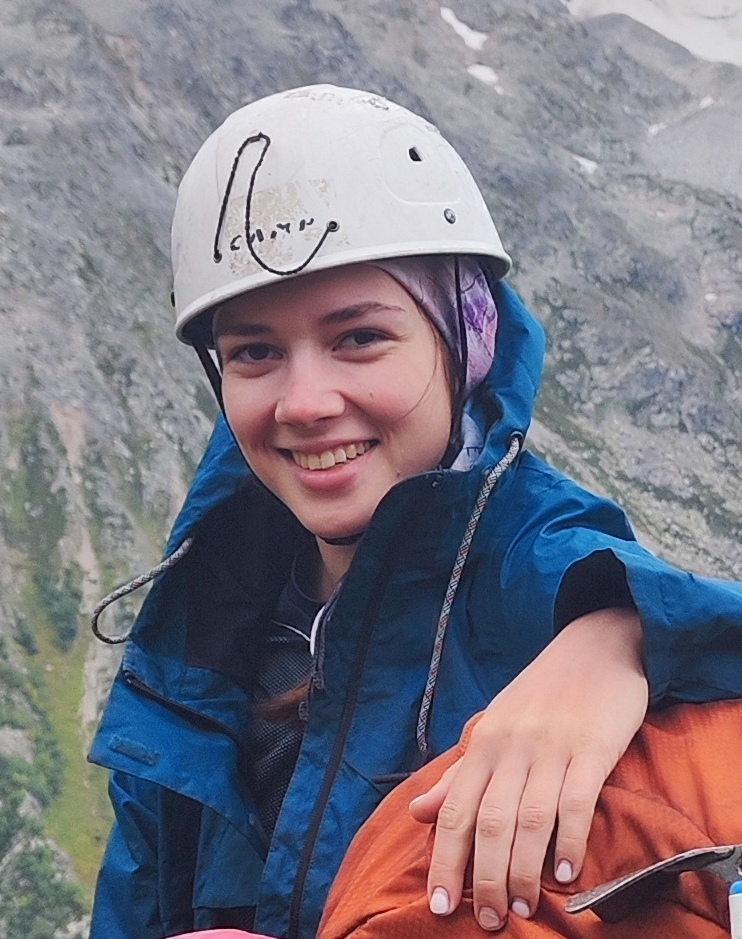
\includegraphics[width=0.99\linewidth]{../pics/portraits/dasha_m}	&	Мерзликина Дарья Сергеевна	&	2000	&	Реммастер	&	1 ст.с. \\
		\hline
		12$^\star$	&	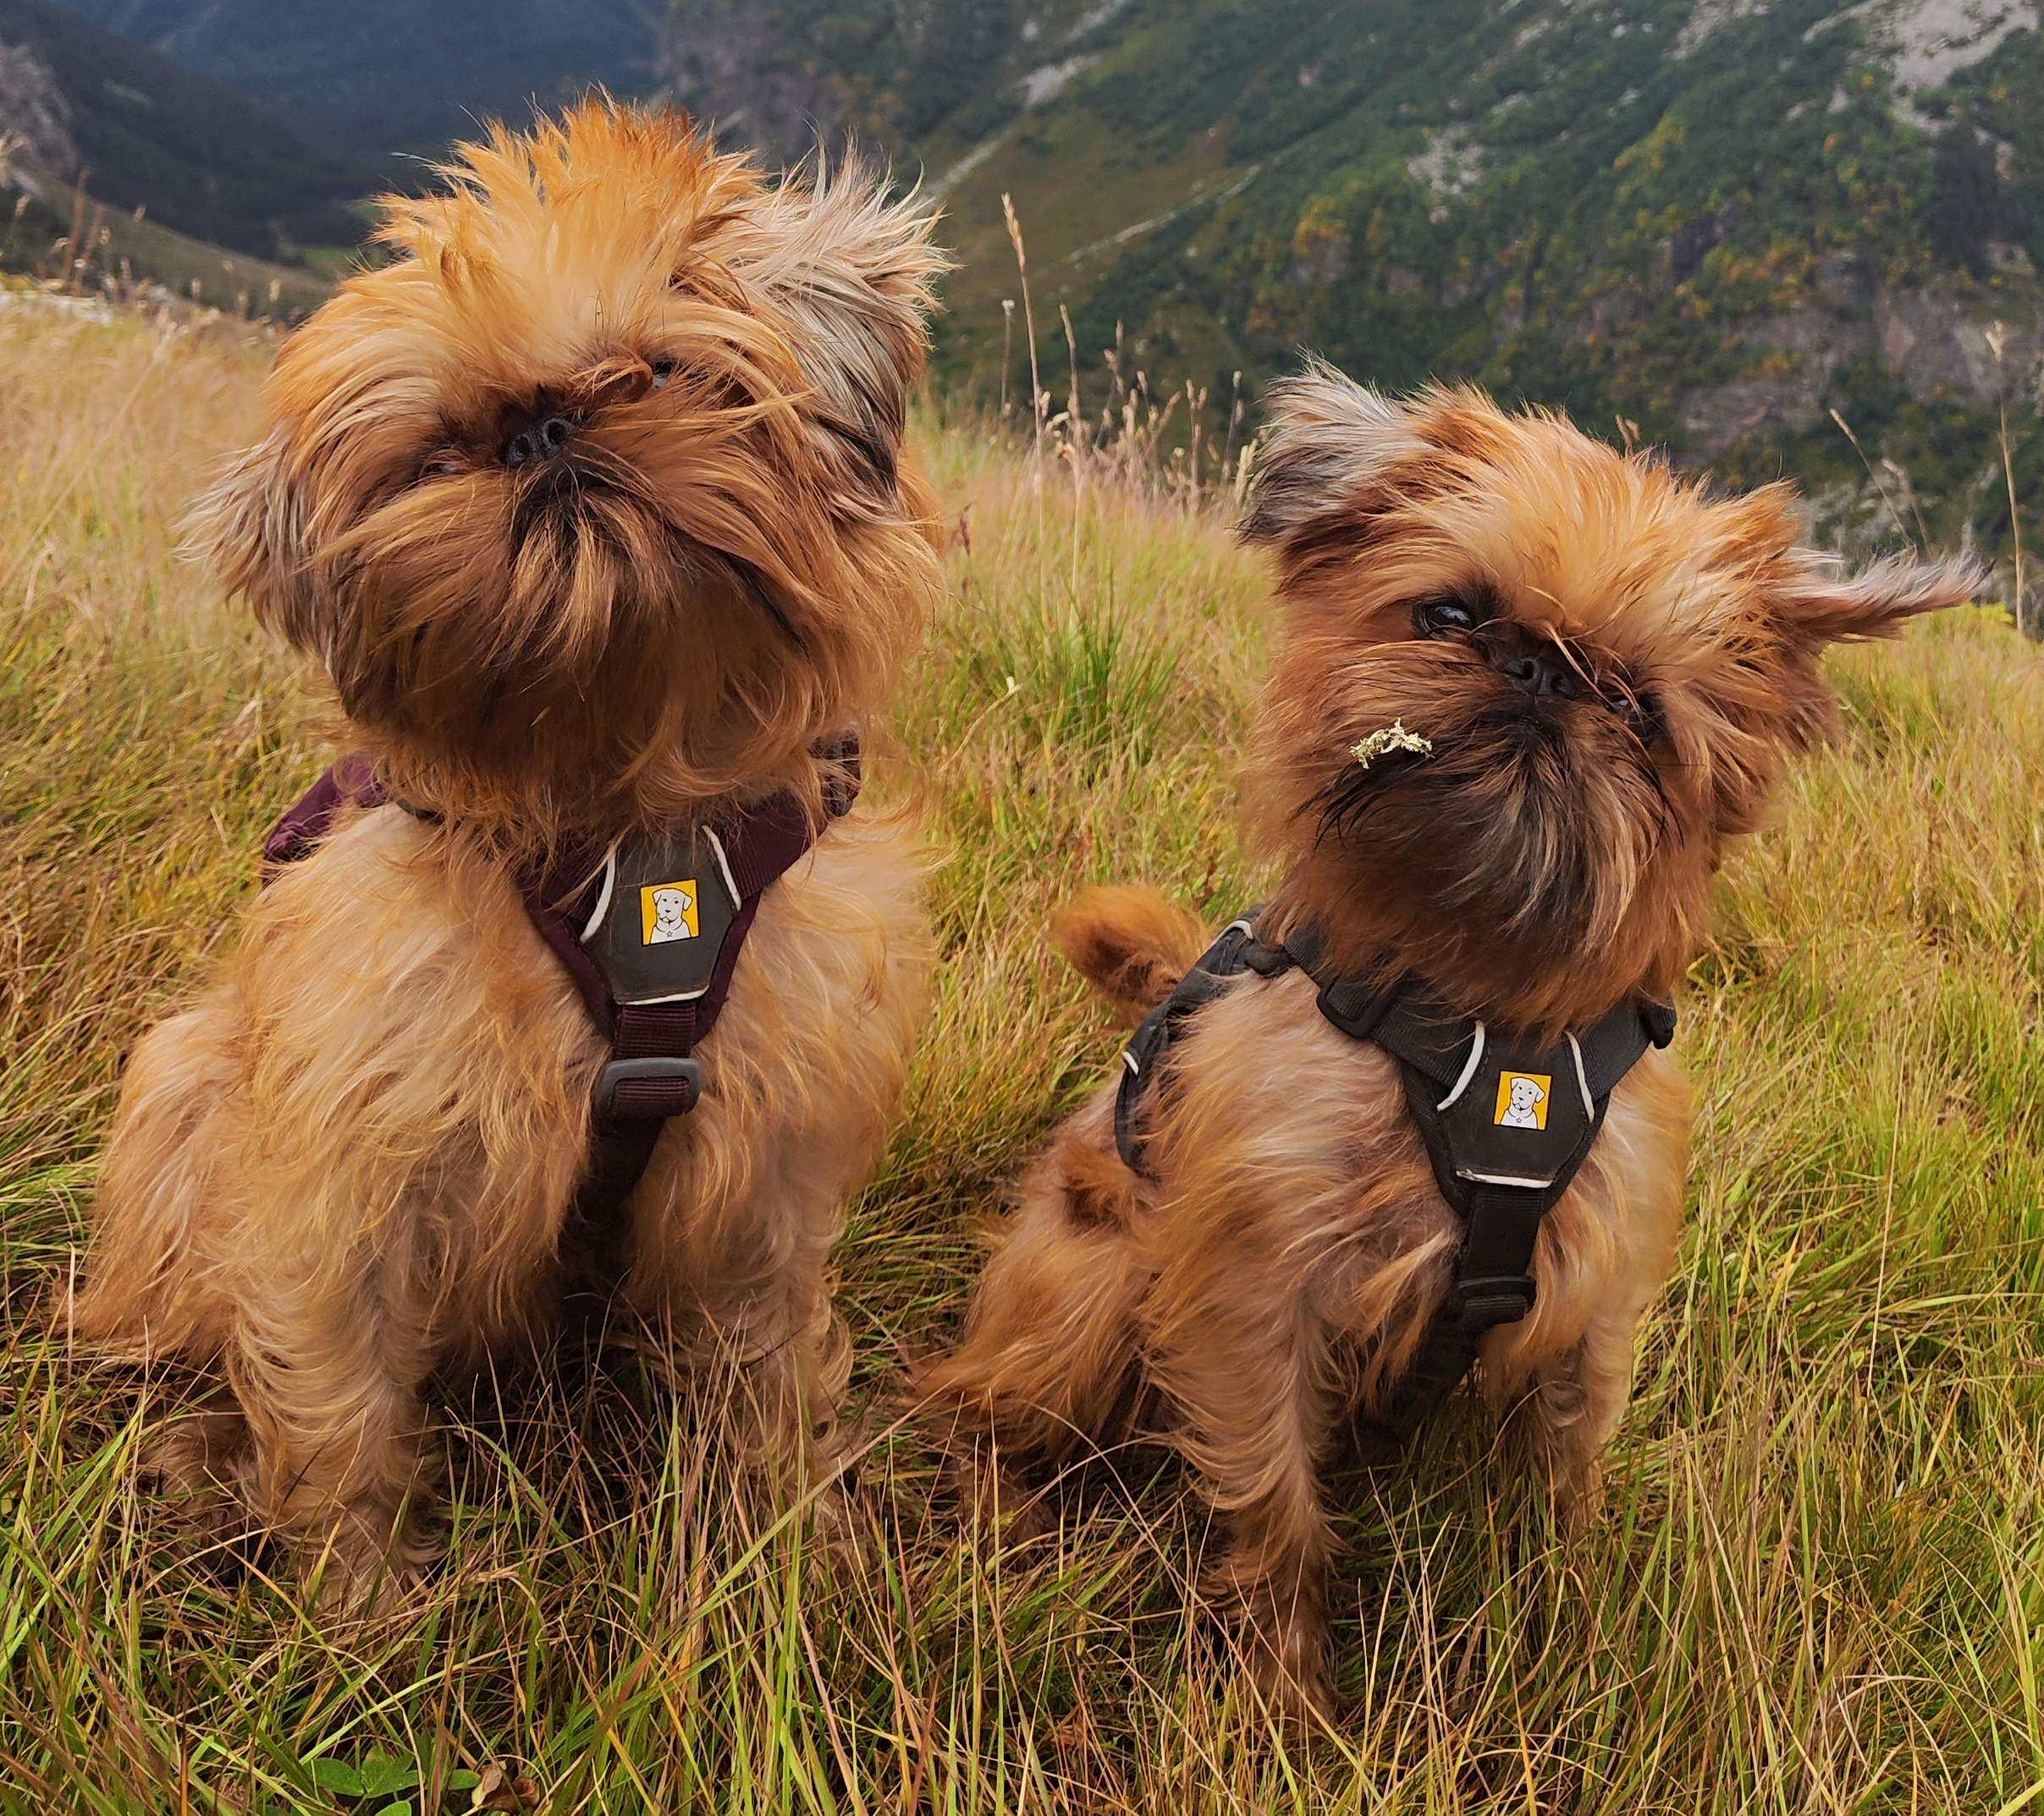
\includegraphics[width=0.8\linewidth]{../pics/portraits/yoshta_aina}	&	Йошта, Айна (брюссельские гриффоны)	&	2022	&	Талисманы команды	&	1 ст.с. \\
		\hline
	\end{tabular}%
	}
\end{table}


%\newpage

\section{Концепт (типа abstract)} 
Тут будет что-то про красоток природы и про то, какая я в целом продуманная молодец.
\section{Литературный обзор}

\subsection{пер. Уллукёль Нижний (н/к, 2933)} 
\subsection{пер. Джалпаккол Северный (1А, ?)} 
\subsection{пер. Кичкинекол Малый (1А, ?)} 
\subsection{пер. Перемётный} 
Пер. Перемётный представляет из себя одно из ключевых и, с точки зрения тактики прохождения, одно из самых сложных препятствий на маршруте. На сайте Вестры \cite{WestraCat} имеется всего пять упоминаний об этом перевале, одно из которых — фотоальбом вершин и перевалов Кавказа за авторством \textcolor{teal}{какого-то чувака, на которого мне сейчас лень ссылаться}, и ещё одно — отчёт Королёва А.~Э. 2018 г. \cite{Korolyov2018}, в котором автор принимал участие, и в ходе которого было решено отказаться от сквозного прохождения Перемётного, заменив его радиальным. \textcolor{teal}{(Попросить Андрея напомнить о причинах!)} Что касается остальных трёх источников, то это отчёты Зеленцовой Е.~А. 2000 г. \cite{Zelentsova2000}, Истягиной Е.~Е. 2015 г. и Анучиной С. 2019 г. \cite{Anuchina2019}: в первых двух пер. Перемётный берётся с запада на восток, из д.~р. Чунгур-джар в д.~р. Талычхан, а в третьем --- с востока на запад, из д.~р. Талычхан в д.~р. Чунгур-джар. 

Основную сложность при прохождении перевала с запада на восток представляет спуск: как в отчёте Зеленцовой, так и в отчёте Истягиной описаны сложности, с которыми сталкивается группа как при планировании спуска, так и в процессе. Обоим руководителям пришлось забирать влево по ходу движения, обходя каньон ручья и мощные скальные выходы, но даже при этом группы Зеленцовой и Истягиной попадали в ловушку из труднопроходимых зарослей рододендрона и берёзового криволесья. Впрочем, после спуска оба автора указывают на возможный оптимальный вариант спуска, который пролегает ещё левее (севернее), в обход криволесья. 

Их выводы полностью подтверждает отчёт Анучиной С. от 2019 г., которая вела группу из трёх человек по каменистому распадку --- руслу пересохшего ручья --- в обход берёзового криволесья. Судя по описанию, этот вариант выглядит довольно щадящим и представляет из себя в основном путь по курумнику с небольшим участком рододендроновых зарослей наверху и высокой травы у подножия склона. В том же отчёте утверждается, что по левому берегу р. Талычхан проходит тропа, которая сливается с тропой, ведущей по левому берегу р. Чунгур-джар. 

Идея взять Перемётный возникла в качестве альтернативы прохождению очень неприятного участка вдоль Чунгурджара: крутого спуска вдоль водопада по заросшему рододендронами склону. Технически на этом склоне имеется тропа, но, по моим воспоминаниям, она легко терялась, и в целом склон был усеян небольшими камнями размером с ботинок, которые невозможно было разглядеть сквозь рододендроновые заросли, и на которых ничего не стоило подвернуть ногу. В случае же с Перемётным мы будем иметь тоже не самый приятный для группы, но более предсказуемый и оттого безопасный спуск по курумнику и обещанную тропу, которая проходит по травянистой долине без большого сброса. Таким образом, я решаю разменять гарантированно неприятный и небезопасный спуск на, предположительно, более долгий, но чуть более безопасный спуск; предположительно терпимую тропу и взятие нового нетривиального перевала с исследованием предположительно оптимального по нему маршрута.

\textcolor{teal}{1. Прописать тайминги по всем трём отчётам (плюс мои прикидки по реверснутому прохождению маршрута Анучиной); 2. Дописаться до Анучиной; 3. Вставить фоточки.}

\subsection{пер. Хотютау (1А, 3546)} 

\appendix
\section{Перевальные записки}
\section{Список снаряжения}
\section{Расходы на группу}

\bibliography{Gvandra2024_Snegovskaya.bib}
\bibliographystyle{plain}



\end{document}